\documentclass{beamer}
\usepackage{lsfolien}
\usepackage[english]{babel}
\usepackage[utf8]{inputenc}

\myfootline{System Modelling and Semantic Web -- Spring 2021}{Hans-Gert Gräbe}

\newcommand{\ueberschrift}[1]{\begin{center}\bf #1\end{center}}

\title{Modelling Sustainable Systems\\ and Semantic Web\\[6pt] Data and
  Information \vskip1em}

\subtitle{Lecture in the Module 10-202-2309\\ for Master Computer Science}

\author{Prof. Dr. Hans-Gert Gräbe\\
\url{http://www.informatik.uni-leipzig.de/~graebe}}

\date{June 2021}
\begin{document}

{\setbeamertemplate{footline}{}
\begin{frame}
  \titlepage
\end{frame}}

\section{The Internet as a World of Fictions}
\begin{frame}{The Internet as a World of Fictions}
  
\ueberschrift{Data and information -- a first approximation}

Bit streams and \textbf{data packets}.
\begin{itemize}
\item There are no bit streams on the "Internet", but rather data packets that
  are sent and received at the devices.  Data packets are generated and
  transformed back again from bit streams at the 4 lower levels of the OSI
  stack.
\item Fiction of the universally networked end devices and reality of the net
  failures.
\end{itemize}
The mouse phenomenon
\begin{itemize}
\item Tools and their use. The spoon.
\item Fictions in everyday life. Discussion.
\end{itemize}\vspace*{2em}
\end{frame}

\begin{frame}{The Internet as a World of Fictions}

\begin{block}{The Notion of Fiction}
  \textbf{Fiction} as socially supported, guaranteed and sustained
  \emph{consensus} on an \emph{abbreviated way of speaking} about a
  \emph{social normality}.
\end{block}
\begin{itemize}
\item Fictions are a specific way of dealing with a increasing complexity of
  the world.
\item Fictions in this sense are not a new phenomenon.
\item Fictions and Myths
  \begin{itemize}
  \item A \emph{myth} in its original meaning is a story. The religious myth
    links human existence with the world of gods or ghosts. Myths demand to be
    valid for the truth they claim. ... The ensemble of all myths of a nation,
    a culture, a religion is called \emph{mythology}.  (Wikipedia)
  \end{itemize}
\end{itemize}
\end{frame}

\begin{frame}{The Internet as a World of Fictions}
\ueberschrift{Complexity and Clock Frequencies in a Society}
\begin{itemize}
\item A clock (or timing) is used to impress a periodicity to a sequence or to
  synchronise processes. The system clock in a computer determines the working
  speed of many components. (Wikipedia)
\item Timing is also essential for the coordination and synchronization of
  social activities.
\item Development of complexity and clock rates of computer chips see
  \url{https://arxiv.org/pdf/1803.00254.pdf}
\item Moore's Law (1965) states that complexity of integrated circuits with
  minimal component costs doubles on a regular basis. Depending on the source,
  the period is 12 to 24 months.
\item But the „human clock rate“ does not change ...
\end{itemize}\vspace*{2em}
\end{frame}

\begin{frame}{The Internet as a World of Fictions}
\ueberschrift{Fiction of the universal end-to-end connection\\ and its
  realization as a scale-free network}\scriptsize
\begin{itemize}
\item $v(k)=c\cdot k^{-a}$ -- proportion of nodes with $k$ neighbors ($v$ as
  valence).
\item Example with $a=3$: $v(1)=0.832$, $v(2)=0.104$, $v(3)=0.031$,
  $v(4)=0.013$, $v(5)=0.007$, $v(6)=0.004$, ...
\item Compared to a random network (another model!) the proportion of
  nodes with many connections (hubs) decreases slower.
\item How quickly does the graph break down into several subgraphs if nodes
  are removed?
\item Scale-free networks are robust against the failure of a larger number of
  randomly selected nodes, but not against failure of a small number of hubs.
\item Robustness: Each node is embedded in a local socio-technical
  infrastructure, which takes care of its operation, maintains the "social
  normality" and thus reproduces the "fiction".
\end{itemize}
\end{frame}

\section{Data and Information}
\begin{frame}{Data and Information}

  \begin{center}
    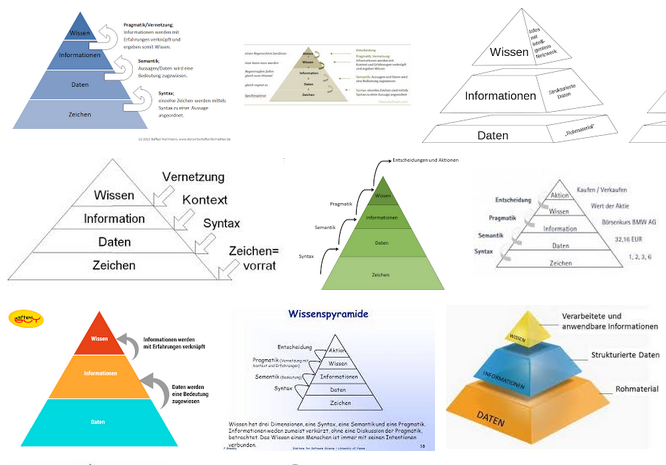
\includegraphics[width=\textwidth]{NuqlkG.png}
  \end{center}
\end{frame}

\begin{frame}{Data and Information}

  \ueberschrift{Syntax, Semantics, Pragmatics}
  
  \begin{block}{Data and Information. A first definition}
    \begin{quote}
      Information = interpreted data\\
      Data = formalized information
    \end{quote}
  \end{block}

Both (formalization and interpretation) are only "valid" in a special natural,
technical or social \emph{embedding} -- a \emph{context} (or pragmatics) --
and thus assume a "working fiction".

Compare this also with the concert example in the first lecture.
\vfill
\end{frame}
\begin{frame}{Data and Information}

  \ueberschrift{Syntax, Semantics, Pragmatics in the OSI layer model}

We consider such a \emph{pragmatically} contextualized interplay of
(formalized) \emph{syntax} and (formalized) \emph{semantics} on different
levels at the example of the OSI stack.

\begin{itemize}
\item Each layer is based on a fiction (i.e., social normality) and its
  language representation given as formalized syntax. 
\item This formalized syntax was practically produced on the previous layer.
\item On this basis a further pragmatics is realised through language
  constructions as special way of speaking (semantics).  
\item This special way of speaking in turn is formalized for use on the next
  layer.
\end{itemize}
\end{frame}

\begin{frame}{Data and Information}
  \begin{center}
    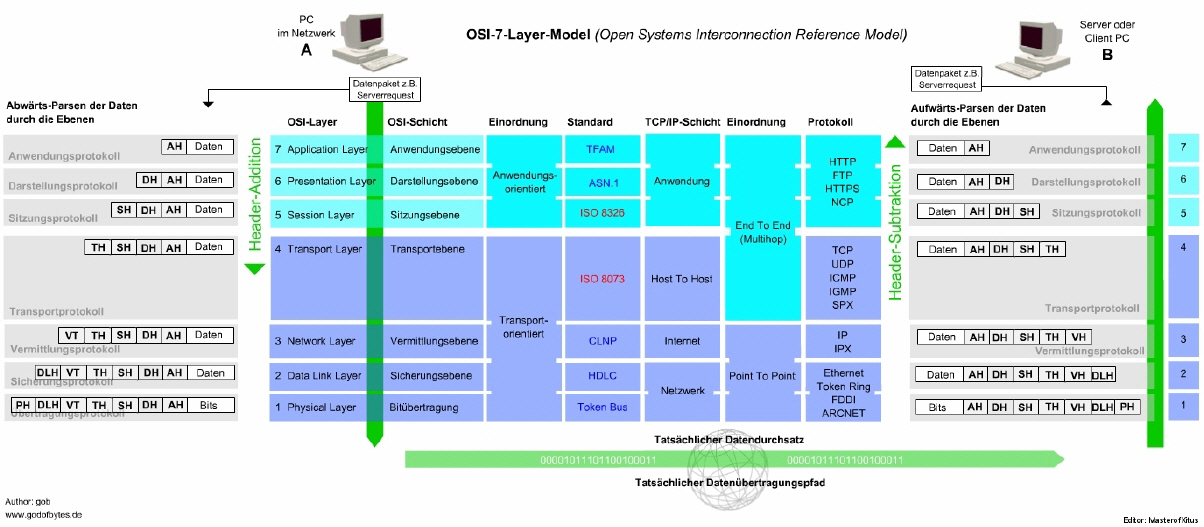
\includegraphics[width=\textwidth]{Rqw330.jpg}
  \end{center}
Source: Wikipedia, \url{http://prima-it.de/images/osi7layermodell.jpg}
\end{frame}
\begin{frame}{Data and Information}

  \ueberschrift{Syntax, Semantics, Pragmatics in the OSI layer model}

\emph{Explanation of this idea:}

Layer 1: 
\begin{itemize}
\item Syntax = modulated waves,
\item Semantics = bit sequences (first fiction), 
\item Pragmatics = diversity of transmission media
\end{itemize}
Layer 2: 
\begin{itemize}
\item Syntax = bit sequences, 
\item Semantics = frames (second fiction),
\item Pragmatics = control of the transmission speed of the bit sequences,
  addition of checksums for error detection
\end{itemize}\vspace*{2em}
\end{frame}
\begin{frame}{Data and Information}

  \ueberschrift{Syntax, Semantics, Pragmatics in the OSI layer model}

Layer 3: 
\begin{itemize}
\item Syntax = frames, 
\item Semantics = data packets (third fiction),
\item Pragmatics = routing and organization of forwarding of packets across
  multiple nodes
\end{itemize}
Etc.\vfill
\end{frame}
\end{document}
